% !TeX spellcheck = id_ID
\documentclass[a4paper,12pt]{article}
\usepackage[bahasa]{babel}
\usepackage{graphicx}
\usepackage{multirow}
\usepackage{enumitem}
\usepackage{listings}
\graphicspath{ {./img/} }
\begin{document}
\title{Laporan Praktikum Statistika Pertemuan 7}
%\author{Aldzikri Dwijayanto Prathama \\ {\small 195410189}}
\author{Aldzikri Dwijayanto Prathama 
	\\195410189}
\makeatletter
\begin{titlepage}
	\begin{center}
		{\huge \bfseries \@title }\\[14ex]
		
\includegraphics[scale=.8]{logo}\\[4ex]
		{\large \@author}\\[20ex]
		{\large \bfseries {SEKOLAH TINGGI MANAJEMEN INFORMATIKA DAN KOMPUTER
				AKAKOM YOGYAKARTA}}
	\end{center}


%{\large \@date} 
\end{titlepage}
\makeatother
%\maketitle
\newpage
\tableofcontents
\newpage
\section{Tujuan}
\begin{enumerate}
	\item Praktikan dapat melakukan penyajian data dalam bentuk tabel Kontingensi
	\item Praktikan dapat melakukan penyajian data dalam bentuk table distribusi Frekuensi
\end{enumerate}
\section{Dasar Teori}
\subsection{Tabel Kontigensi}
\paragraph{}
Tabel Kontigensi merupakan tabel yang digunakan untuk mengukur hubungan (asosiasi) antara dua variable kategorik dimana tabel tersebut merangkum frekuensi bersama dari observasi pada setiap kategori variable. 
\paragraph{}
Misalkan n sampel diklasifikasikan secara silang berdasarkan dua atribut atau lebih dalam suatu.
\paragraph{}
Berikut ini contoh tabel kontingesi 2x2 :
\begin{table}[!ht]
	\begin{tabular}{|c|c|l|l|c|}
		\hline
		\multicolumn{2}{|l|}{\multirow{2}{*}{}} & \multicolumn{2}{l|}{Variable 2}                 & \multirow{2}{*}{Total} \\ \cline{3-4}
		\multicolumn{2}{|l|}{}                  & \multicolumn{1}{c|}{1} & \multicolumn{1}{c|}{2} &                        \\ \hline
		\multirow{2}{*}{Variable 1}     & 1     & $O_{11}$                       &$O_{12}$                      &\multicolumn{1}{l|}{$n_{1+}$ }  \\ \cline{2-5} 
		& 2     & $O_{21}$                       & $O_{22}$                       & \multicolumn{1}{l|}{$n_{2+}$}  \\ \hline
		\multicolumn{2}{|c|}{Total}             & $n_{+1}$                       &  $n_{+2}$                      & N                      \\ \hline
	\end{tabular}
\end{table}
\paragraph{}
Dengan menggunakan R Console maka :
\begin{enumerate}
	\item Untuk membuat Tabel \textit{Contingency} dua arah dengan Fungsi \textit{\textbf{table( )}} dari  \textit{data.frame}
	\item Untuk membuat Tabel Contingency tiga Arah atau lebih dengan Fungsi \textit{\textbf{ftable( )}} untuk membentuk tabel contingency tiga arah dari \textit{data.frame}.
\end{enumerate}
\subsection{Distribusi Frekuensi}
\paragraph{}
Distribusi frekuensi adalah daftar nilai data (bisa nilai individual atau nilai data yang sudah dikelompokkan ke dalam selang interval tertentu) yang disertai dengan nilai frekuensi yang sesuai.
\paragraph{}
Pengelompokkan data ke dalam beberapa kelas dimaksudkan agar ciri-ciri penting data tersebut dapat segera terlihat. Daftar frekuensi ini akan memberikan gambaran yang khas tentang bagaimana keragaman data.
\paragraph{}
Distribusi frekuensi dibuat dengan alasan berikut:
\begin{enumerate}[label=\alph*.]
	\item kumpulan data yang besar dapat diringkas
	\item kita dapat memperoleh beberapa gambaran mengenai karakteristik data, dan
	\item merupakan dasar dalam pembuatan grafik penting (seperti histogram).
\end{enumerate}
\paragraph{}
Pada saat menyusun tabel distribusi frekuensi, pastikan bahwa 
\begin{enumerate}[label=\alph*.]
	\item kelas tidak tumpang tindih sehingga setiap nilai-nilai pengamatan harus masuk tepat ke dalam satu kelas
	\item tidak akan ada data pengamatan yang tertinggal (tidak dapat dimasukkan ke dalam kelas tertentu). 
\end{enumerate}
\paragraph{}
Dengan menggunakan R Console maka :
\begin{enumerate}
	\item Penyajian data dalam bentuk tabel  distribusi frequensi dapat digunakan \textbf{fungsi \textit{table()}}
	\item Untuk  penyajian data dalam bentuk tabel  distribusi frequensi relatif  digunakan \textbf{fungsi \textit{table()/length()}}
	\item Untuk Membuat Tabel Distribusi Frekuensi untuk Data Berkelompok digunakan \textbf{fungsi \textit{cut( )}} untuk membuat suatu interval. Argumen \textbf{\textit{break}} digunakan untuk menentukan batas-batas interval.	
\end{enumerate}
\section{Praktik}
\subsection{Tabel Kontigensi}
\subsubsection{Praktik 1}
\paragraph{Soal\\}
Sajikan data berikut ini dalam bentuk table kontigensi 
\begin{table}[!ht]
	\begin{tabular}{|c|c|}
		\hline 
		Pendidikan & Jenis Kelamin \\ 
		\hline 
		S1 & Laki-laki \\ 
		\hline 
		S1 & Laki-laki \\ 
		\hline 
		S1 & Laki-laki \\ 
		\hline 
		S1 & Perempuan \\ 
		\hline 
		S1 & Perempuan \\ 
		\hline 
		S2 & Perempuan \\ 
		\hline 
		S2 & Perempuan \\ 
		\hline 
		S2 & Perempuan \\ 
		\hline 
		S2 & Perempuan \\ 
		\hline 
		S2 & Laki-laki \\ 
		\hline 
	\end{tabular}
\end{table} 
\paragraph{Penyelesaian\\}
Buat variabel dan masukkan data dari variabel tersebut dengan dengan fungsi c dengan format perintah\\ 
\texttt{>variabel <- c("data 1","data 2"..."data n").}\\
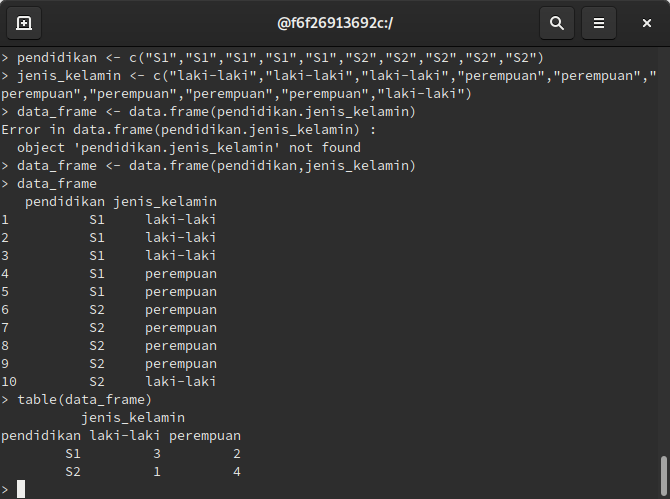
\includegraphics[width=\linewidth]{1}\\
Pada praktik ini dibuat variabel \texttt{pendidikan}, yang berisi data jenjang pendidikan, dan variabel \texttt{jenis\_kelamin} yang berisi jenis kelamin.\\
Seteleh itu dibuat tabel kontigensi dua arah dari variabel \texttt{data\_frame}, dengan perintah\\
\texttt{>table(data\_frame)}
\subsubsection{Praktik 2}
\paragraph{Soal\\}
Sajikan data berikut ini dalam tabel kontigensi
\begin{table}[!ht]
	\begin{tabular}{|l|l|l|l|l|}
		\hline
		No & Jenis\_kelamin & \multicolumn{1}{c|}{Pendidikan} & \multicolumn{1}{c|}{status} & \multicolumn{1}{c|}{hobi} \\ \hline
		1  & Laki-laki      & S1                              & Sudah menikah               & membaca                   \\ \hline
		2  & Laki-laki      & S1                              & Sudah menikah               & membaca                   \\ \hline
		3  & Laki-laki      & S1                              & Belum menikah               & membaca                   \\ \hline
		4  & Perempuan      & S1                              & Sudah menikah               & membaca                   \\ \hline
		5  & Perempuan      & S1                              & Sudah menikah               & memasak                   \\ \hline
		6  & Perempuan      & S2                              & Belum menikah               & membaca                   \\ \hline
		7  & Perempuan      & S2                              & Sudah menikah               & membaca                   \\ \hline
		8  & Perempuan      & S2                              & Belum menikah               & memasak                   \\ \hline
		9  & Perempuan      & S2                              & Belum menikah               & membaca                   \\ \hline
		10 & Laki-laki      & S2                              & Sudah menikah               & memasak                   \\ \hline
	\end{tabular}
\end{table}
\paragraph{Penyelesaian\\}
Buat variabel dan masukkan data dari variabel tersebut dengan format perintah\\ \texttt{>variabel <- c("data 1","data 2"..."data n").}\\
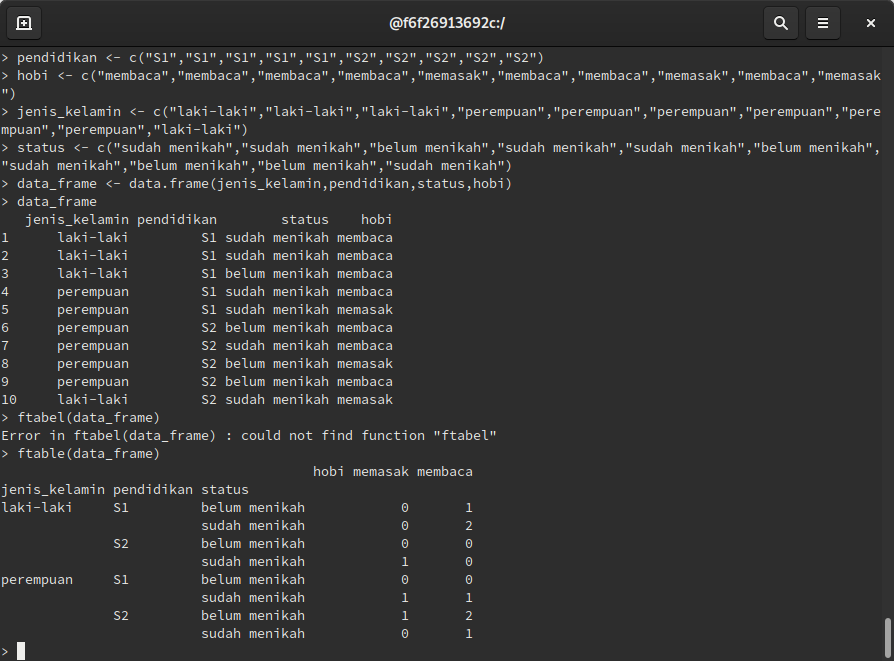
\includegraphics[width=\linewidth]{2}\\
Untuk praktek ini buat variabel \texttt{pendidikan} dan masukkan data dari pendidikan ke variabel tersebut dengan fungsi \texttt{c}\\
Selanjutnya buat variabel \texttt{hobi}, \texttt{jenis\_kelamin}, dan \texttt{status} lalu beri data sesuai klasifikasi variabel tersebut.\\
Lalu buat data frame yang terdiri dari variabel \texttt{jenis\_kelamin}, \texttt{pendidikan}, \texttt{status}, \texttt{hobi} dengan nama data\_frame,dengan perintah\\ 
\texttt{>data\_frame <- data.frame(jenis\_kelamin,pendidikan,status,hobi)}\\
lalu buat tabel kontigensi dari tabel data\_frame, karena lebih dari dua arah maka tidak menggunakan perintah \texttt{table}, gunakan perintah\\
\texttt{>ftable(data\_frame)}

\subsection{Distribusi Frekuensi}
\subsubsection{Praktik 1}
\paragraph{Soal\\}
Dari data berikutini sajikan dalam bentuk tabel distribusi frekuensi dan tabel distribusi frekuensi relatif. Data : 1, 2, 3, 2, 3, 3, 4, 5, 3, 2, 3, 4, 5, 5, 5, 5, 3, 2, 1, 3.\\
\paragraph{Penyelesaian\\}
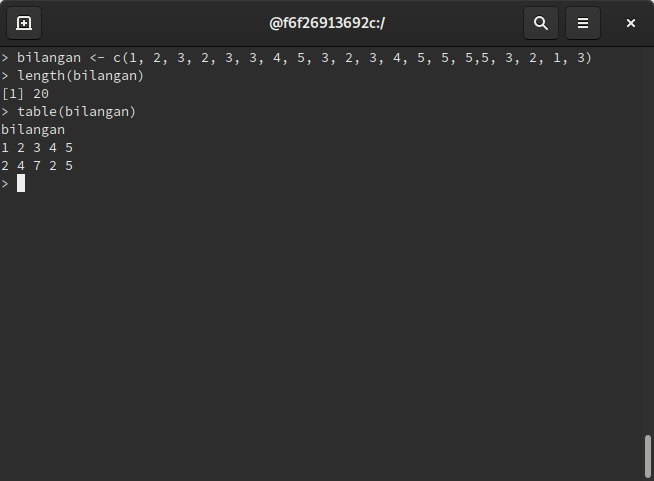
\includegraphics[width=\linewidth]{3}
Buat variabel \texttt{bilangan}, dan masukkan dengan fungsi \texttt{c}, dengan perintah\\
\texttt{>bilangan <- c(1, 2, 3, 2, 3, 3, 4, 5, 3, 2, 3, 4, 5, 5, 5, 5, 3, 2, 1, 3)\\}
cek banyaknya data pada variabel \texttt{bilangan} dengan perintah\\
\texttt{>length(bilangan)}\\
lalu buat tabel distribusi frekuensi dari variabel \texttt{bilangan} dengan perintah\\
\texttt{>table(bilangan)}
\subsubsection{Praktik 2}
\paragraph{Soal\\}
Sajikan data berikut dalam bentuk tabel distribusi frekuensi\\ 
1, 2, 3, 4, 5, 6, 7, 8, 9, 10, 10, 9, 8, 4, 3, 2\\ 
Kelas intervalnya 1 – 4, 5 - 10\\
\paragraph{Penyelesaian\\}
Buat variabel \texttt{bilangan} dan masukkan data menggunakan fungsi \texttt{c}\\
\texttt{>bilangan <- c(1, 2, 3, 4, 5, 6, 7, 8, 9, 10, 10, 9, 8, 4, 3, 2)}
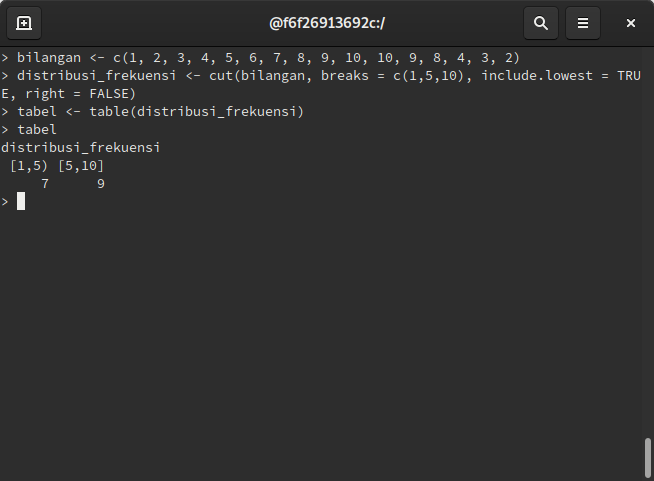
\includegraphics[width=\linewidth]{4}
\section{Latihan}
\subsection{Latihan 1}
\paragraph{Soal\\}
Berikut ini data mahasiswa\\
\begin{table}[!ht]
	\begin{tabular}{|c|c|c|}
		\hline 
		nama & {gender} & {jurusan} \\ 
		\hline 
		Toni & Pria & D3 TI \\ 
		\hline 
		Tino & Pria & S1 SI \\ 
		\hline 
		Ana & Wanita & D3 MI \\ 
		\hline 
		Ina & Wanita & D3 TI \\ 
		\hline 
		Windha & Wanita & S1 TI \\ 
		\hline 
		Mega & Wanita & D3 MI \\ 
		\hline 
		Arif & Pria & S1 SI \\ 
		\hline 
		Tono &  Pria & D3 TI \\ 
		\hline 
		Linda & Wanita & D3 TI \\ 
		\hline 
		Paijo & Pria & S1 TI \\ 
		\hline 
	\end{tabular}
\end{table}\\
Tentukan:
\begin{enumerate}
	\item Tabel distribusi frekuensi mahasiswa menurut jurusannya
	\item Tabel distribusi frekuensi mahasiswa menurut gendernya
\end{enumerate}
\paragraph{Penyelesaian\\}
Pada latihan ini, saya memasukkan data menggunakan fungsi \texttt{read.table}, pertama buat tabel dalam text editor, dan diberi nama mahasiswa.txt.\\
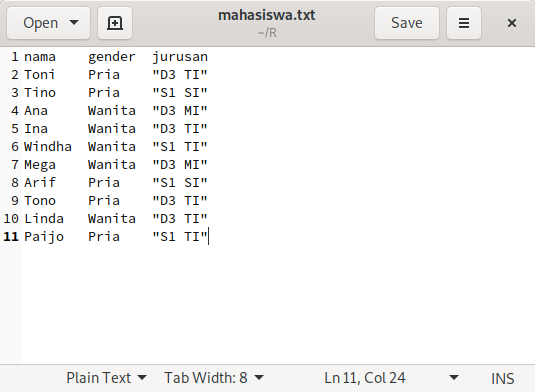
\includegraphics[width=\linewidth]{mahasiswatxt}
Setelah itu masukkan tabel tersebut ke variabel \texttt{mahasiswa} beserta headernya\\
\texttt{>mahasiswa <- read.table("mahasiswa.txt",header=T)}.\\
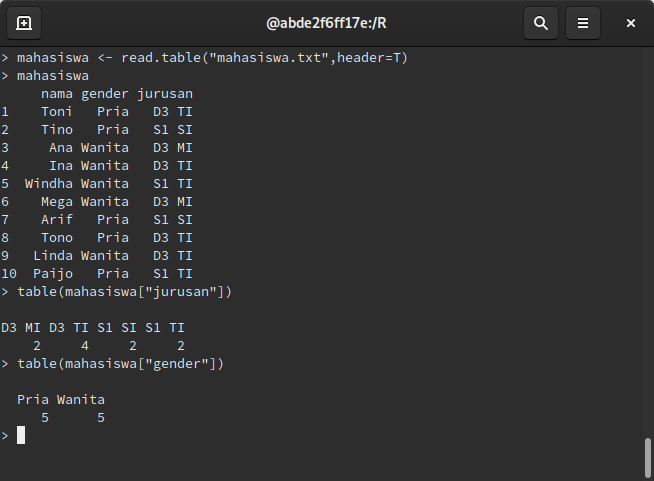
\includegraphics[width=\linewidth]{5}
Untuk membuat tabel distribusi frekuensi mahasiswa menurut jurusan berarti kita akan memakai tabel jurusan dan mengambil data dari kolom jurusan, gunakan perintah\\
\texttt{>table(mahasiswa["jurusan"])}\\
Sedangkan untuk tabel distribusi frekuensi mahasiswa menurut gendernya berarti kita akan memakai tabel jurusan dan mengambil data dari kolom gender, gunakan perintah\\
\texttt{>table(mahasiswa["gender"])}\\
\newpage 
\subsection{Latihan 2}
\paragraph{Soal\\}
Sajikan data berikuta dalam tabel kontigensi
\begin{table}[!ht]
	\begin{tabular}{|l|l|l|l|}
		\hline
		\multicolumn{1}{|c|}{Jenis Kelamin} & \multicolumn{1}{c|}{Bidang} & \multicolumn{1}{c|}{Status} & \multicolumn{1}{c|}{Didik} \\ \hline
		Laki-laki                           & Marketing                   & Belum menikah               & SMU                        \\ \hline
		Perempuan                           & Marketing                   & Sudah menikah               & Sarjana                    \\ \hline
		Perempuan                           & Umum                        & Sudah menikah               & SMU                        \\ \hline
		Laki-laki                           & Akuntansi                   & Belum menikah               & Sarjana                    \\ \hline
		Perempuan                           & Marketing                   & Sudah menikah               & SMU                        \\ \hline
		Perempuan                           & Akuntansi                   & Sudah menikah               & Sarjana                    \\ \hline
		Perempuan                           & Akuntansi                   & Belum menikah               & Sarjana                    \\ \hline
		Laki-laki                           & Umum                        & Belum menikah               & Sarjana                    \\ \hline
		Perempuan                           & Marketing                   & Sudah menikah               & SMU                        \\ \hline
		Laki-laki                           & Marketing                   & Sudah menikah               & SMU                        \\ \hline
	\end{tabular}
\end{table}
\paragraph{Penyelesaian\\}
Buat tabel dalam text editor\\
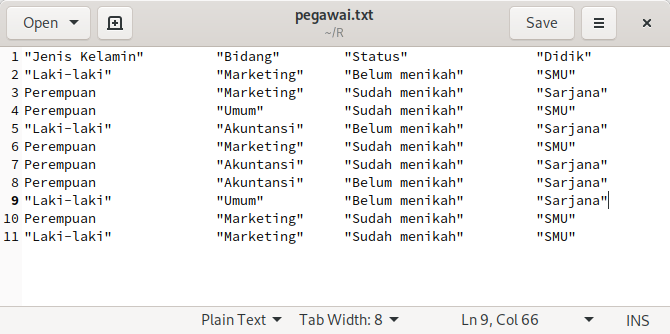
\includegraphics[width=\linewidth]{pegawaitxt}
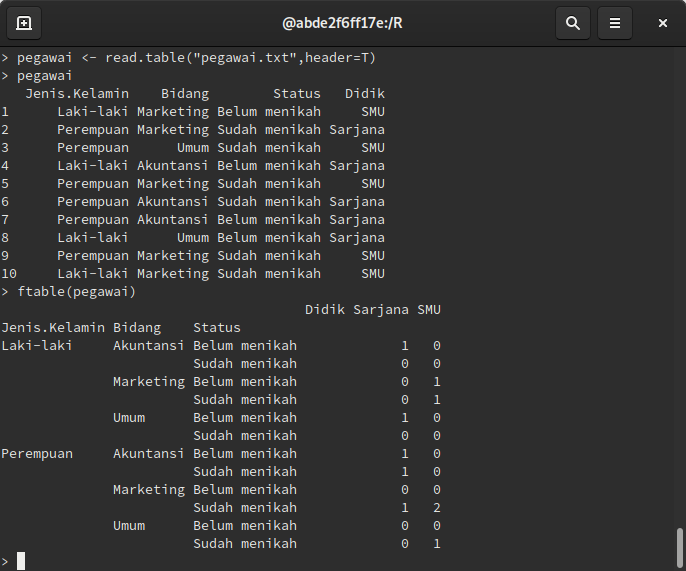
\includegraphics[width=\linewidth]{6}
masukkan tabel tadi ke dalam variabel \texttt{pegawai} dengan headernya menggunakan fungsi \texttt{read.table}\\
\texttt{>pegawai <- read.table("pegawai.txt",header=T)}\\
lalu buat tabel kontigensi dari variabel \texttt{pegawai}\\
\texttt{>ftable(pegawai)}
\newpage
\section{Tugas}
\subsection{Tugas 1}
\paragraph{Soal\\}
Sajikan data tersebut dalam bentuk tabel kontigensi
\begin{table}[!ht]
	\begin{tabular}{|l|l|}
		\hline
		\multicolumn{1}{|c|}{Daerah} & \multicolumn{1}{c|}{Barang} \\ \hline
		Bandung                      & Komputer                    \\ \hline
		Solo                         & TV                          \\ \hline
		Bandung                      & Komputer                    \\ \hline
		Bandung                      & TV                          \\ \hline
		Yogya                        & Radio                       \\ \hline
		Bandung                      & Komputer                    \\ \hline
		Solo                         & TV                          \\ \hline
		Solo                         & Radio                       \\ \hline
		Solo                         & Radio                       \\ \hline
		Bandung                      & TV                          \\ \hline
		Bandung                      & Komputer                    \\ \hline
		Solo                         & Radio                       \\ \hline
		Bandung                      & Radio                       \\ \hline
		Bandung                      & TV                          \\ \hline
	\end{tabular}
\end{table}
\paragraph{Penyelesaian\\}
Buat tabel ke dalam file .txt menggunakan text editor.\\
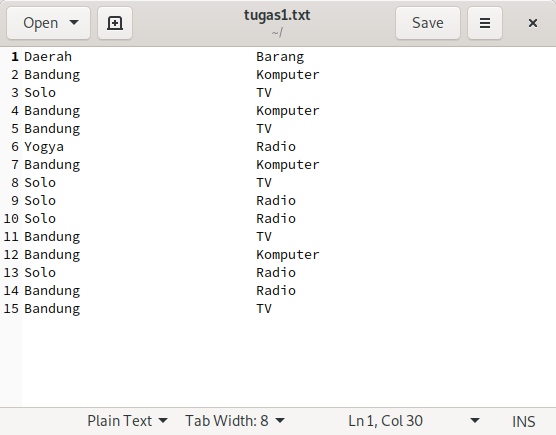
\includegraphics[width=\linewidth]{tugas1txt}
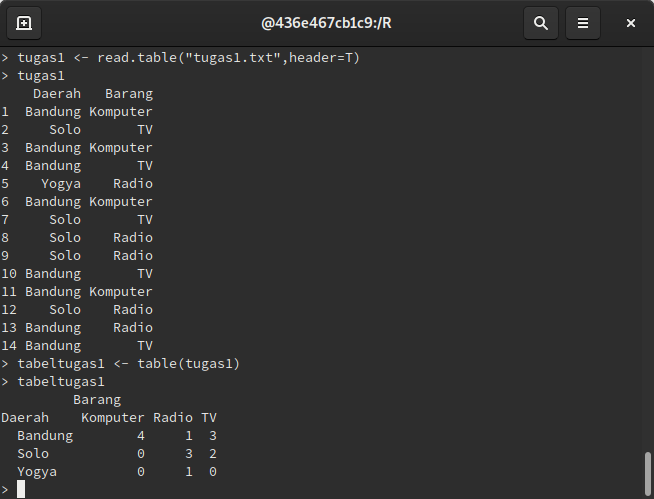
\includegraphics[width=\linewidth]{tugas1output}

\end{document}